\lstinputlisting[language=bash,basicstyle=\small]{python_codes/fieldstone_52/keywords}

\begin{center}
Code at \url{https://github.com/cedrict/fieldstone/tree/master/python_codes/fieldstone_52}
\end{center}

\par\noindent\rule{\textwidth}{0.4pt}

%%%%%%%%%%%%%%%%%%%%%%%%%%%%%%%%%%%%%%%%%%%%%%%%%%%%%%%%%%%%%%%%%%%%%%%%%%%%%%%%%%%%%%%

The domain is a unit square and we solve the mms problem 'VJ3' (see Section~ \ref{mms10}):
\begin{eqnarray}
u(x,y) &=& 200x^2(1-x)^2y(1-y)(1-2y) \nn\\
v(x,y) &=& -200x(1-x)(1-2x)y^2(1-y)^2 \nn\\
p(x,y) &=& 10\left[(x-1/2)^3y^2+(1-x)^3(y-1/2)^3 \right] -5/4 \nn
\end{eqnarray}
The 5/4 term in the pressure equation insures that the pressure is exactly zero in the 
upper right corner (this boundary condition is implemented to get rid of 
the pressure nullspace). It is also the value of the average pressure over the domain.



We will look at three second order elements:
\begin{itemize}
\item The Taylor-Hood $Q_2\times Q_1$ 
\item The serendipity element $Q_2^{(8)}\times Q_1$. The shape functions 
and their derivatives are in Section~\ref{sec:serendipity2D}.
\item A modified serendipity element by 
Zhang \& Xiang (2020) \cite{zhxi20}, the $QH8-C1 \times Q_2$.
\end{itemize}

The global numbering of nodes for both types of elements is shown  
in this simple $4\times 3$ element mesh:

\begin{verbatim}
      Q_2 X Q1 (serendipity)                    Q_2 X Q_1 (regular)

15--47--16--48--17--49--18--50--19      54--55--56--57--58--59--60--61--62
 |       |       |       |       |       |   :   |   :   |   :   |   :   |
42      43      44      45      46      45..46..47..48..49..50..51..52..53
 |       |       |       |       |       |   :   |   :   |   :   |   :   |
10--38--11--39--12--40--13--41--14      36--37--38--39--40--41--42--43--44
 |       |       |       |       |       |   :   |   :   |   :   |   :   |
33      34      35      36      37      27..28..29..30..31..32..33..34..35
 |       |       |       |       |       |   :   |   :   |   :   |   :   |
05--29--06--30--07--31--08--32--09      18--19--20--21--22--23--24--25--26
 |       |       |       |       |       |   :   |   :   |   :   |   :   |
24      25      26      27      28      09..10..11..12..13..14..15..16..17
 |       |       |       |       |       |   :   |   :   |   :   |   :   |
00--20--01--21--02--22--03--23--04      00--01--02--03--04--05--06--07--08

iel= 0:                                  iel= 0
node  0 : 0 at pos. 0.0 0.0              node  0 : 0 at pos. 0.0 0.0
node  1 : 1 at pos. 1.0 0.0              node  1 : 2 at pos. 1.0 0.0
node  2 : 6 at pos. 1.0 1.0              node  2 : 20 at pos. 1.0 1.0
node  3 : 5 at pos. 0.0 1.0              node  3 : 18 at pos. 0.0 1.0
node  4 : 20 at pos. 0.5 0.0             node  4 : 1 at pos. 0.5 0.0
node  5 : 25 at pos. 1.0 0.5             node  5 : 11 at pos. 1.0 0.5
node  6 : 29 at pos. 0.5 1.0             node  6 : 19 at pos. 0.5 1.0
node  7 : 24 at pos. 0.0 0.5             node  7 : 9 at pos. 0.0 0.5
                                         node  8 : 10 at pos. 0.5 0.5
\end{verbatim}

We see that the serendipity element-based mesh counts only 51 nodes, as
opposed to 63 for its counterpart.
Setting $nelx=nely$, we can look at the number of velocity nodes for each 
as a function of $nelx$, as shown hereunder:

\begin{center}
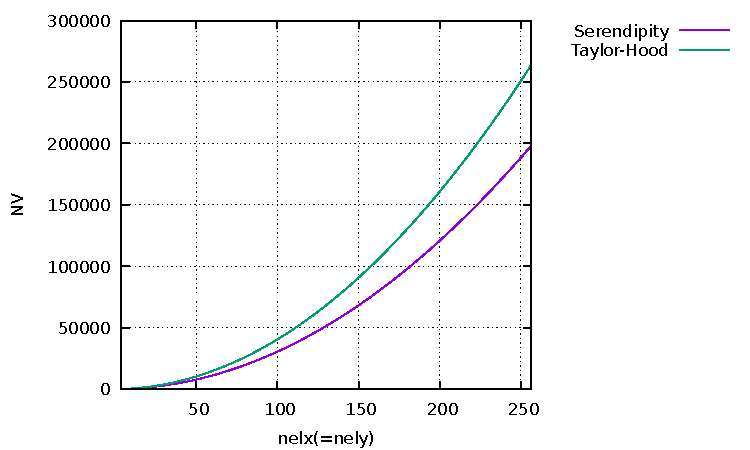
\includegraphics[width=6cm]{python_codes/fieldstone_52/images/NV.pdf}
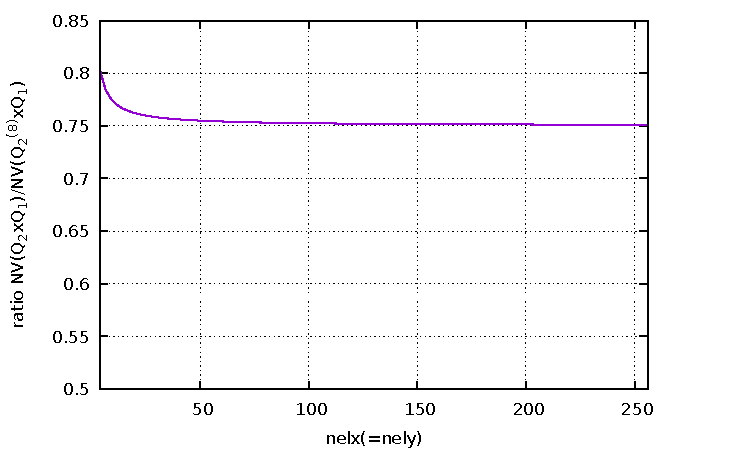
\includegraphics[width=6cm]{python_codes/fieldstone_52/images/NV_ratio.pdf}\\
{\captionfont Left: NV for both elements as a function of nelx. Right: ratio of the 
two.}
\end{center}
Looking at the ratio between both, we see that ultimately 
at high resolution, a mesh composed of serendipity elements 
will count 25\% less nodes than a mesh with Taylor-Hood elements.
Since there is not free lunch, what is the price paid in terms of accuracy when using 
the cheaper serendipity? 

Although the vtk format does not support the $Q_2$ element in 2D or 3D, it surprisingly does
support the serendipity element in 2D (type=23) and 3D (type=25).

Two types of grids are generated. The first one is a mesh composed of square (or rectangular)
elements. The second one has random noise added to the first one: the position of each corner 
node (with the exception of those on the domain boundaries) is perturbed by a randomly computed 
(positive or negative) distance equal to $0.1h$ at the maximum. Note that the nodes
on the edges between corner nodes are relocated to the middle of the edge so as to generate
straight-side quadrilaterals.

\begin{center}
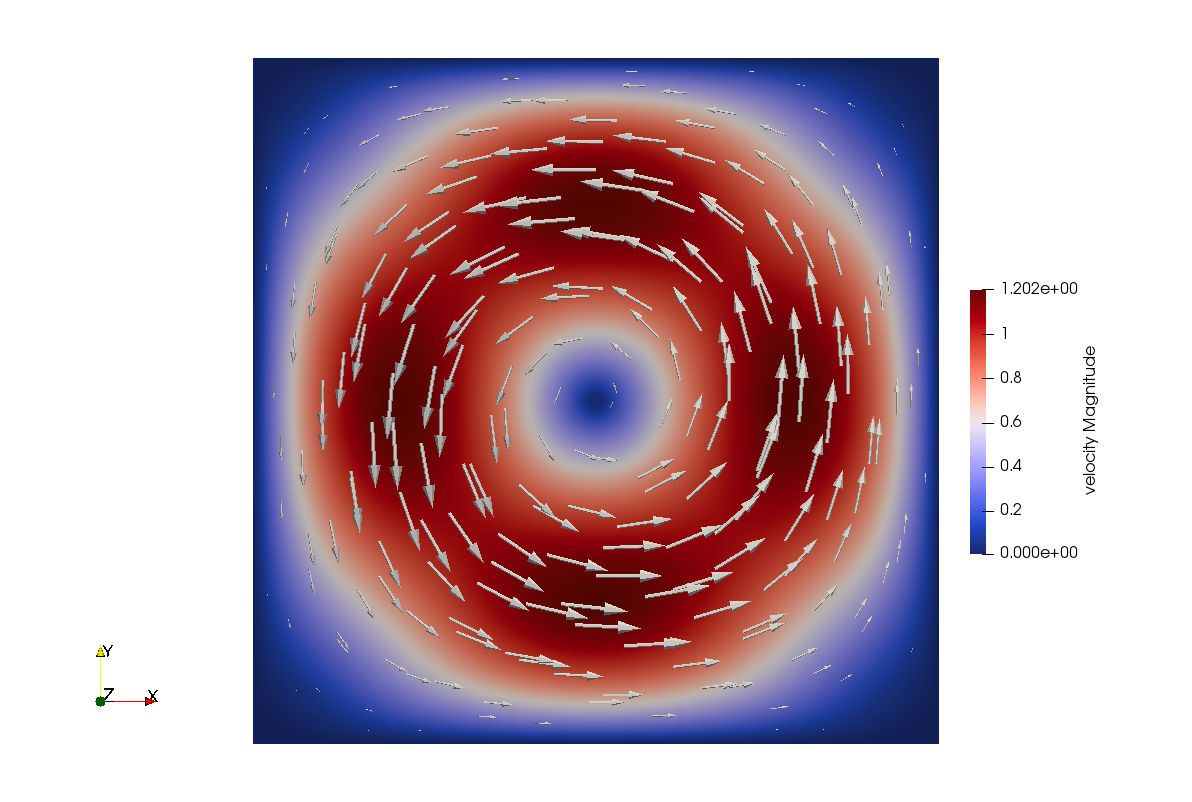
\includegraphics[width=7cm]{python_codes/fieldstone_52/images/vel}
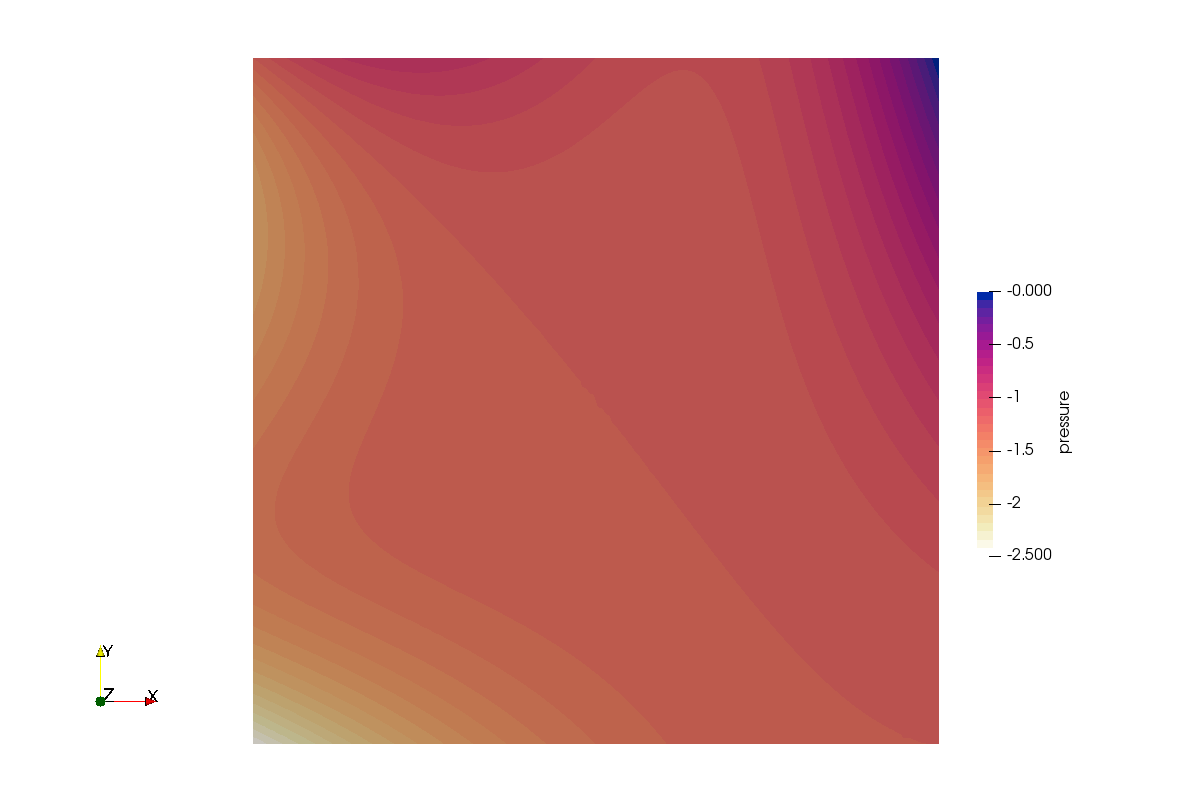
\includegraphics[width=7cm]{python_codes/fieldstone_52/images/press}
\end{center}


We then compute the velocity and pressure error as a function of resolution $h$:

\begin{center}
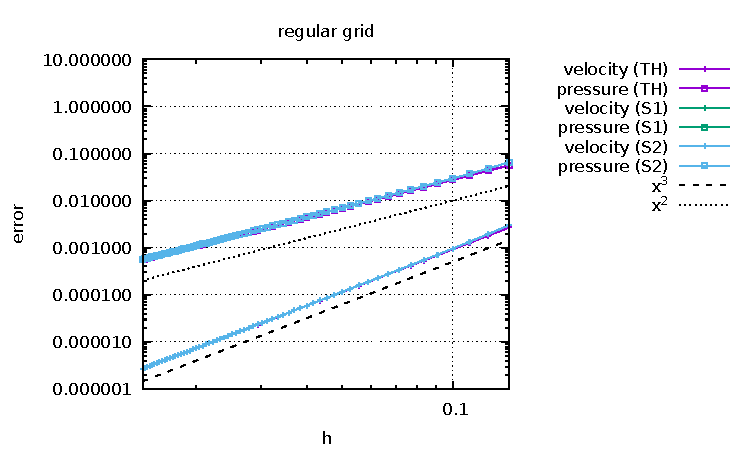
\includegraphics[width=7.8cm]{python_codes/fieldstone_52/images/errors_reg.pdf}
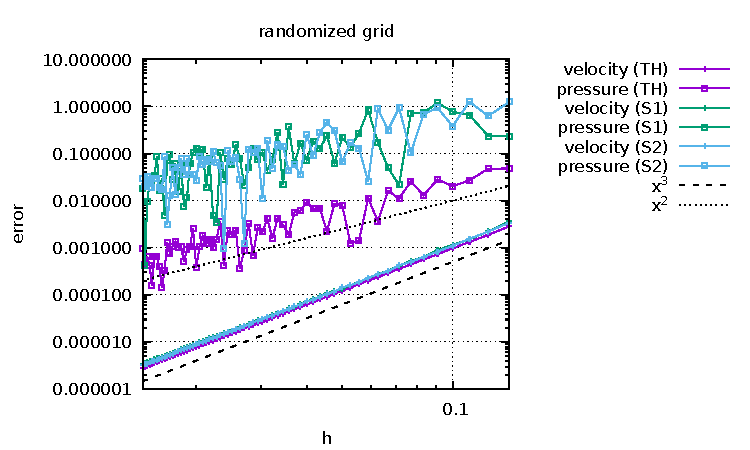
\includegraphics[width=7.8cm]{python_codes/fieldstone_52/images/errors_rand.pdf}\\
{\captionfont 'TH' is Taylor-Hood, 'S1' is serendipity $Q_2^{(8)}\times Q_1$, 'S2' is $QH8C1\times Q_1$ element.}
\end{center}

Note that the $QH8C1\times Q_1$ element is identical to the regular $Q_2^{(8)}\times Q_1$ element 
in the case of regular meshes since in this case $m_x=m_y=0$, so that its results are the same as those 
of the regular serendipity element. 

For regular grids the serendipity element yields the same errors and error convergence 
rates as its Taylor-Hood counterpart. Since it is cheaper in terms of dofs, 
one could think that it should be preferred. However, most modern codes 
use an iterative solver approach to solve the discretised Stokes problem, and 
often the $\K$ matrix (which is SPD) is 'solved' with a conjugate gradient solver.  
The convergence of this type of solver depends on the condition number of the matrix
itself, i.e. the ratio of the largest and smallest eigenvalues. 
Note that this is rather trivial with Python:

\begin{lstlisting}
print('condition number:', nel,linalg.cond(K_mat))
\end{lstlisting}
However, since I was also curious about the values of the eigenvalues, I implemented 
it as follows:
\begin{lstlisting}
eigvals, eigvecs = linalg.eig(K_mat)
print('eigenvalues:',nel,eigvals.min(),eigvals.max())
\end{lstlisting}

\begin{center}
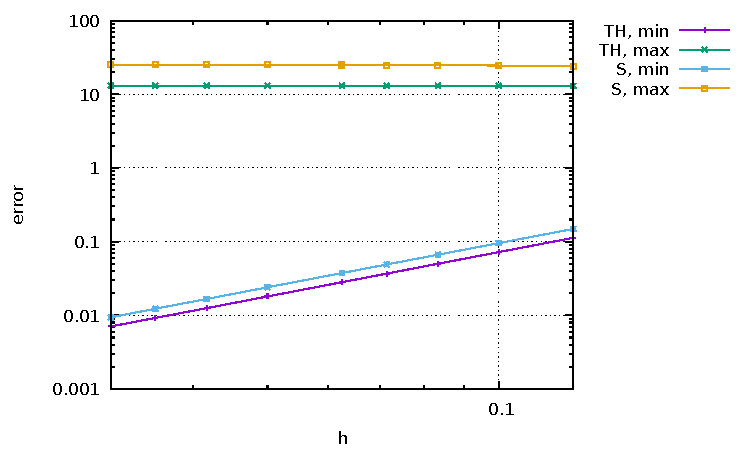
\includegraphics[width=6cm]{python_codes/fieldstone_52/images/eigenvalues.pdf}
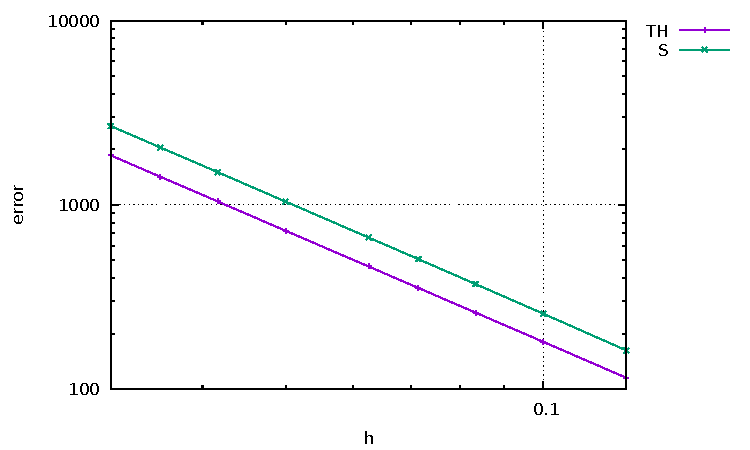
\includegraphics[width=6cm]{python_codes/fieldstone_52/images/eigenvalues_ratio.pdf}\\
{\captionfont Left: min and max eigenvalues for both types of elements as a function of $h$; 
Right: condition number}
\end{center}
As it turns out, the condition number is twice as high for the serendipity element, 
which means that the CG would have to iterate more to arrive at the solution, 
thereby offsetting the benefit of less dofs.

Looking back at the error rates for the randomised grids we see that the error 
velocity is virtually unchanged. Even though the pressure error still decreases 
quadratically with the mesh size, it does now do so in a much more erratic way. 
Also the Taylor-Hood element outperforms the serendipity elements by about an 
order of magnitude. 



